\documentclass[12pt,german]{article}

\usepackage[left=2cm, right=2cm, top=2cm, bottom=3.5cm, landscape=false]{geometry}

\usepackage{graphicx}
\usepackage{float}
\usepackage[flushleft]{threeparttable}

\usepackage{tabularx}
\newcolumntype{R}{>{\raggedleft\arraybackslash}X}
\newcolumntype{L}{>{\raggedright\arraybackslash}X}
\newcolumntype{C}{>{\centering\arraybackslash}X}
\usepackage{booktabs}
\usepackage{dcolumn}

\usepackage[ngerman]{babel}

\usepackage{amsmath}

\title{\vspace{-1.5cm}Protokoll Bildung und Zerfall}
\author{Fuchs, Gutmann, Kosbab, Kowal, Steindorf, Fälker, Richter}

\begin{document}
    \maketitle
    \tableofcontents

    \section{Kurzbeschreibung des Versuches}
    \begin{itemize}
        \item Zu Beginn des Versuchs wird ohne Probe fünf mal der Nulleffekt gemessen und aus den erhaltenen Werten der Durchschnittswert gebildet.
        \item Ein Aluminium-Präparat, ein Kupfer-Präparat sowie ein unbekanntes Präparat werden für jeweils 10 Minuten im geöffneten Experimentierkanal bestrahlt.
        \item Nach erfolgter Neutronen-Aktivierung werden die Proben aus dem Reaktorkanal entnommen und in den Szintillator montiert.
        \item Anschließend wird über eine Zeitdauer von 10 Minuten alle 30 Sekunden die Zahl der Impulse für je sechs Sekunden gemessen.
    \end{itemize}

    \section{Funktionsweise eines Szintillators}
    \begin{enumerate}
        \item Im Szintillationskristall des Szintillators werden beim Auftreffen von Strahlung Lichtblitze (Szintillationen) erzeugt.
        \item Die Lichtblitze werden in einem Sekundärelektronenverstärker durch den fotoelektrischen Effekt in Fotoelektronen umgewandelt und durch Stoßionisation verstärkt.
        \item Die enstehenden Spannungsimpulse werden in einem nachfolgenden Verstärker weiter verstärkt und anschließend im Impulszähler gezählt.
    \end{enumerate}
    Folgende Werte wurden am Strahlungsmessgerät eingestellt:
    \begin{table}[H]
        \centering
        \begin{tabularx}{0.7\textwidth}{L|R}
            \toprule
            \textbf{Parameter} & \textbf{Wert} \\
            \midrule
            Pegel & $5.7\, V$ \\
            Hochspannung & $-1140\, V$ \\
            Verstärkung & $22\, dB$ \\
            Messzeit & $6\, s$ \\
            Kanalbreite & DIS \\
            \bottomrule
        \end{tabularx}
    \end{table}

    \section{Nullwertmessungen}
    \begin{table}[H]
        \begin{tabularx}{\textwidth}{R|R|R}
            \toprule
            \raggedright\textbf{Messung} & \raggedright\textbf{Messwert ohne Menschen} & \multicolumn{1}{l}{\textbf{Messwert mit Menschen}} \\
            & $[\#\, Impulse]$ & $[\#\, Impulse]$ \\
            \midrule
            1 & 522 & 408 \\
            2 & 522 & 488 \\
            3 & 545 & 415 \\
            4 & 526 & 396 \\
            5 & 575 & 492 \\
            \midrule
            \O & $N_0$ = 538 & 439,8 \\
            \bottomrule
        \end{tabularx}
        \caption{Untergrundstrahlung bei laufendem Reaktor mit und ohne Menschen als Abschirmmaterial}
    \end{table}

    \section{Messwerte}
    \begin{table}[H]
        \begin{threeparttable}
        \begin{tabularx}{\textwidth}{L|R|R|R|R|R|R}
            \toprule
            \textbf{Zeit} & \multicolumn{2}{c|}{\textbf{Al $[\#\, Impulse]$}} & \multicolumn{2}{c|}{\textbf{Cu $[\#\, Impulse]$}} & \multicolumn{2}{c}{\textbf{X $[\#\, Impulse]$}} \\
            $[min]$ & \multicolumn{1}{c}{$N_i$} & \multicolumn{1}{c|}{$N_i - N_0$} & \multicolumn{1}{c}{$N_i$} & \multicolumn{1}{c|}{$N_i - N_0$} & \multicolumn{1}{c}{$N_i$}$N_i$ & \multicolumn{1}{c}{$N_i - N_0$} \\
            \midrule
            0 & 27845* & 27307* & 24197* & 23659* & 12051* & 11513*   \\
            0,5 & 24505 & 23967 & 24063 & 23525 & 11971 & 11433   \\
            1,0 & 21163 & 20625 & 22350 & 21812 & 11134 & 10596   \\
            1,5 & 18339 & 17801 & 20668 & 20130 & 10651 & 10113   \\
            2,0 & 15840 & 15302 & 19868 & 19330 & 10252 & 10113   \\
            2,5 & 13718 & 13180 & 18376 & 17838 & 9285  & 8747    \\
            3,0 & 11656 & 11118 & 17582 & 17044 & 8809  & 8271    \\
            3,5 & 10279 & 9741  & 16477 & 15939 & 8314  & 7776    \\
            4,0 & 8744  & 8206  & 15461 & 14923 & 8117  & 7579    \\
            4,5 & 7612  & 7074  & 14629 & 14097 & 7423  & 6885    \\
            5,0 & 6536  & 5998  & 13838 & 13300 & 7081  & 6543    \\
            5,5 & 5961  & 5423  & 12893 & 12355 & 6791  & 6253    \\
            6,0 & 5102  & 4564  & 12004 & 11466 & 6380  & 5842    \\
            6,5 & 4426  & 3888  & 11673 & 11135 & 6026  & 5488    \\
            7,0 & 3948  & 3410  & 11196 & 10658 & 5638  & 5100    \\
            7,5 & 3381  & 2843  & 10355 & 9817  & 5410  & 4872    \\
            8,0 & 3060  & 2522  & 10077 & 9539  & 5180  & 4642    \\
            8,5 & 2691  & 2153  & 9477  & 8939  & 4852  & 4314    \\
            9,0 & 2300  & 1762  & 9009  & 8471  & 4645  & 4107    \\
            10,0 & 1930 & 1392  & 8152  & 7614   & 4096  & 3558   \\
            \bottomrule
        \end{tabularx}
        \begin{tablenotes}
            \small
            \item * durch exponentielle Extrapolation berechnet
        \end{tablenotes}
        \caption{Anzahl der Impulse für verschiedene Materialien zu verschiedenen Zeitpunkten}
    \end{threeparttable}
    \end{table}

    \section{Graphische Darstellung}
    % Fehlerbetrachtung Henry
    \begin{figure}[H]
        \centering
        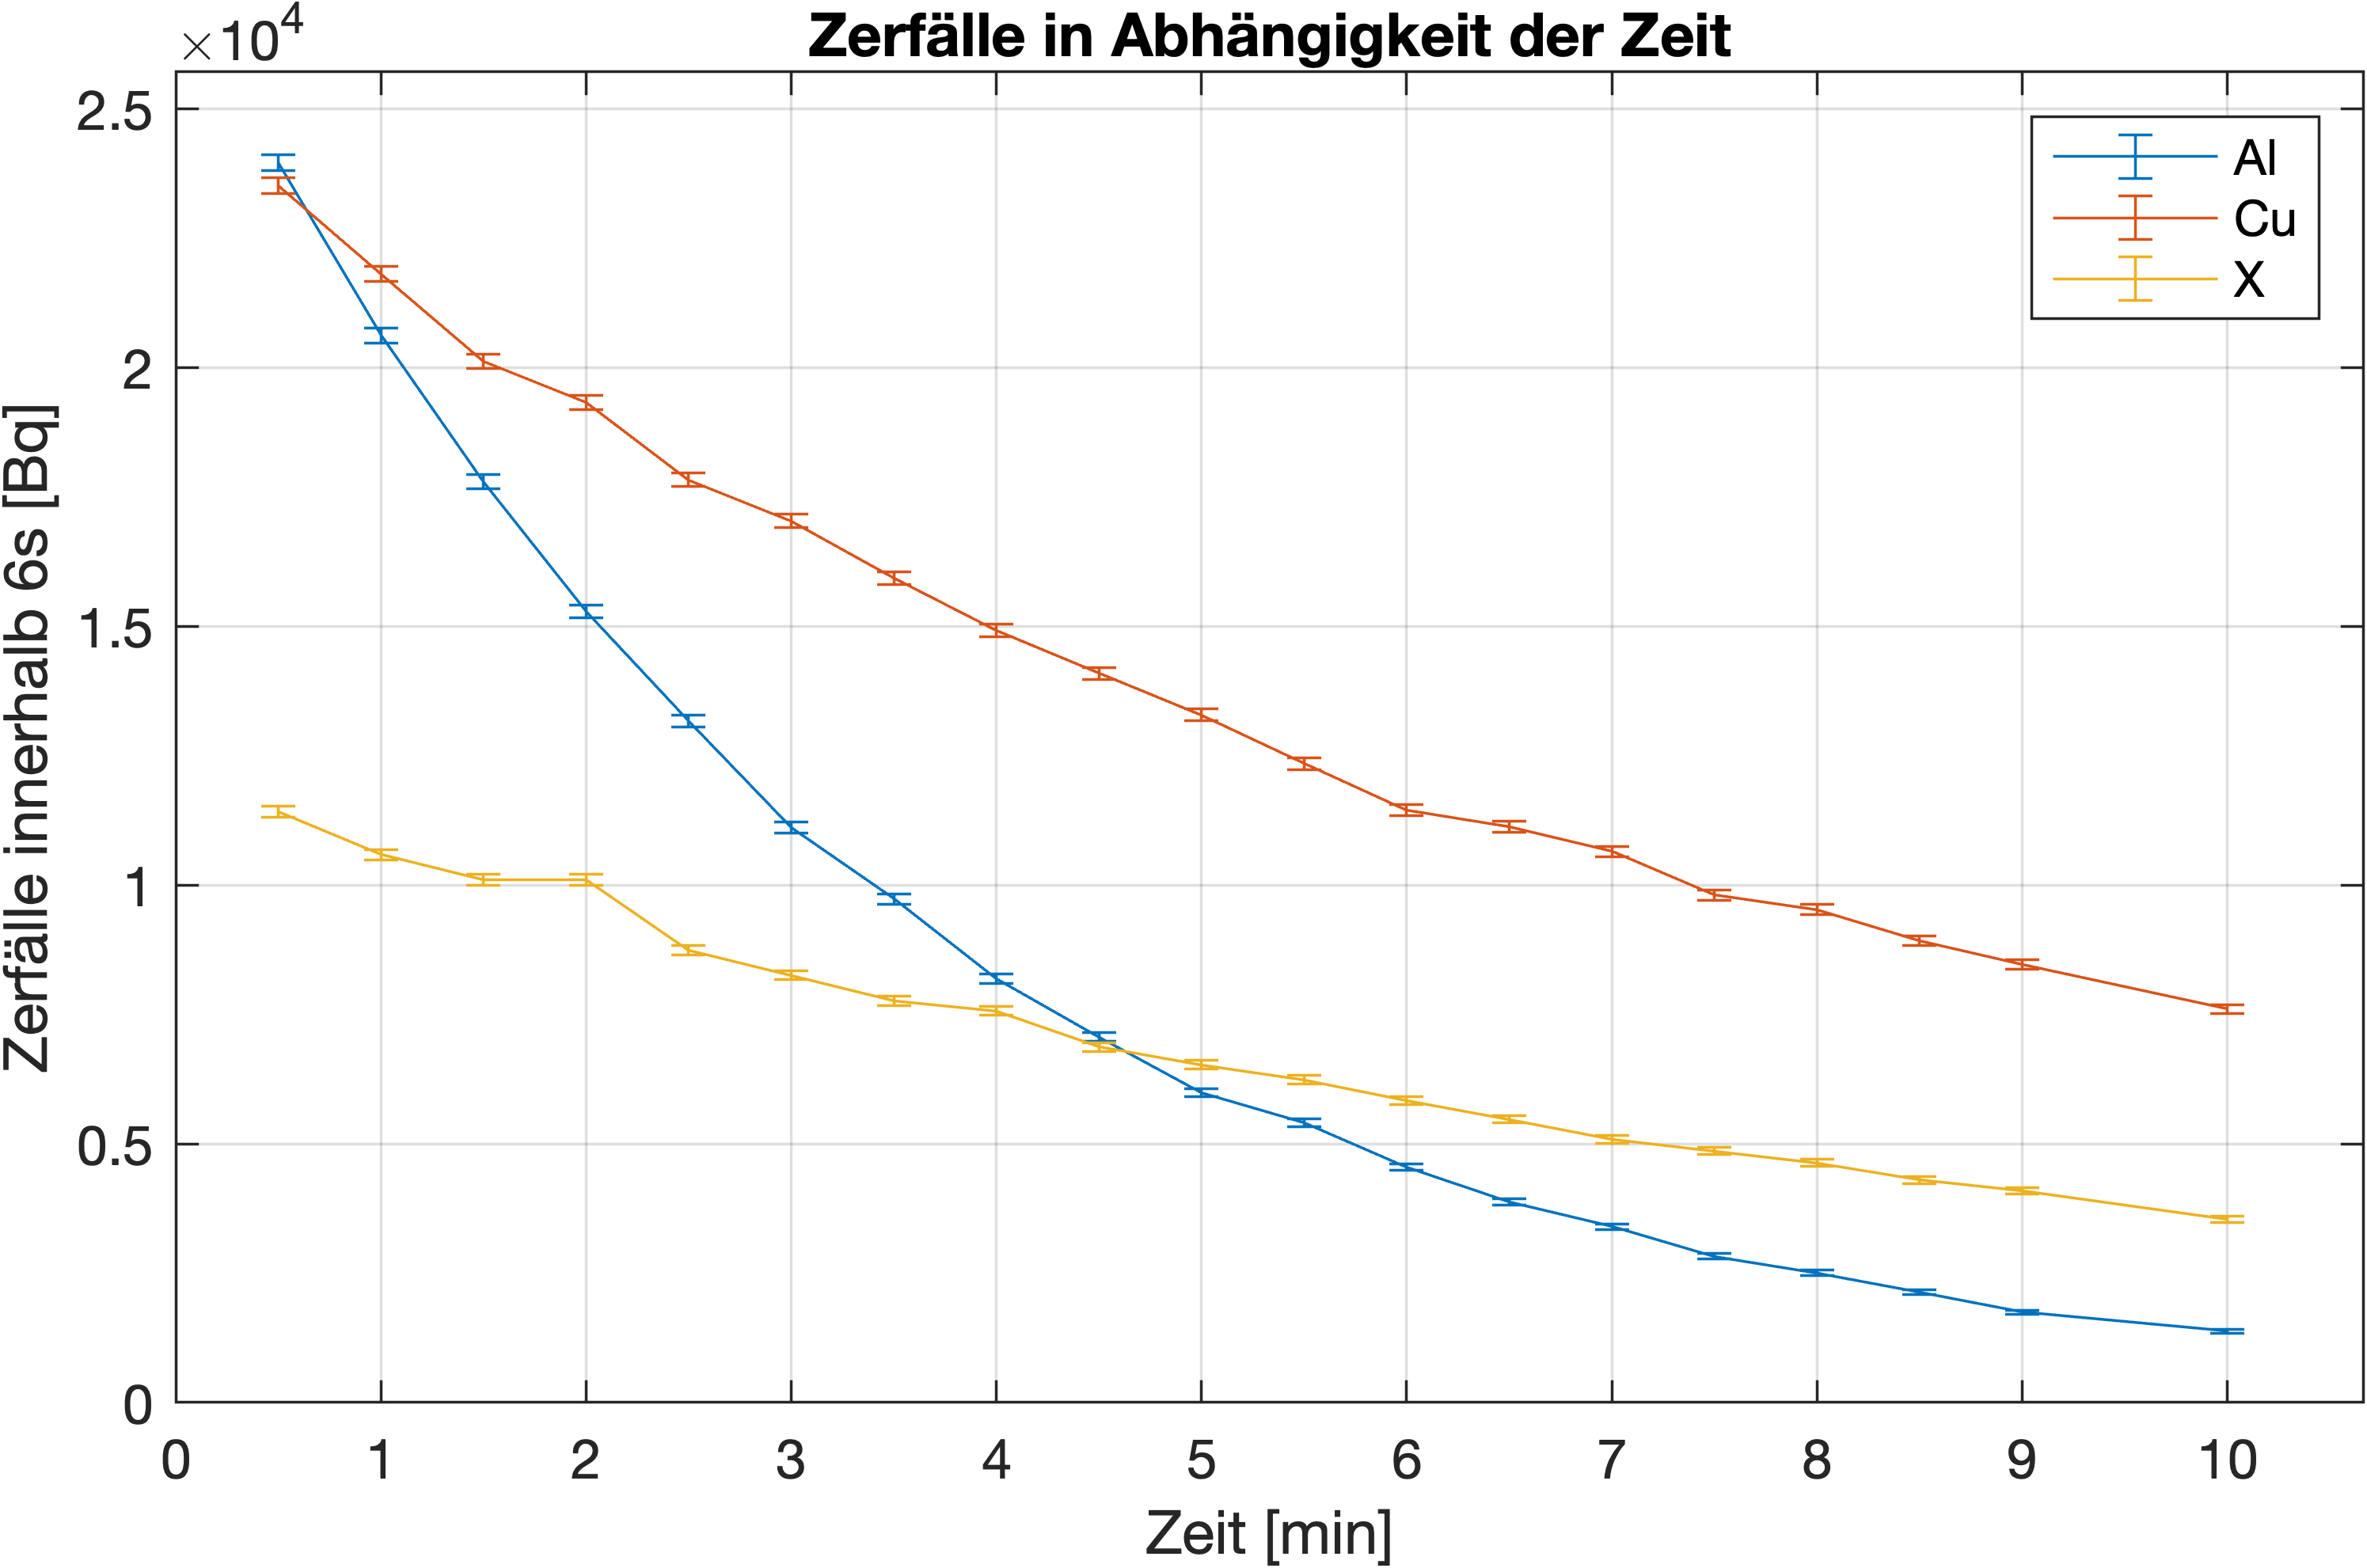
\includegraphics[width=\textwidth]{linear.png}
        \caption{Messwerte mit linearer Achse}
    \end{figure}
    \begin{figure}[H]
        \centering
        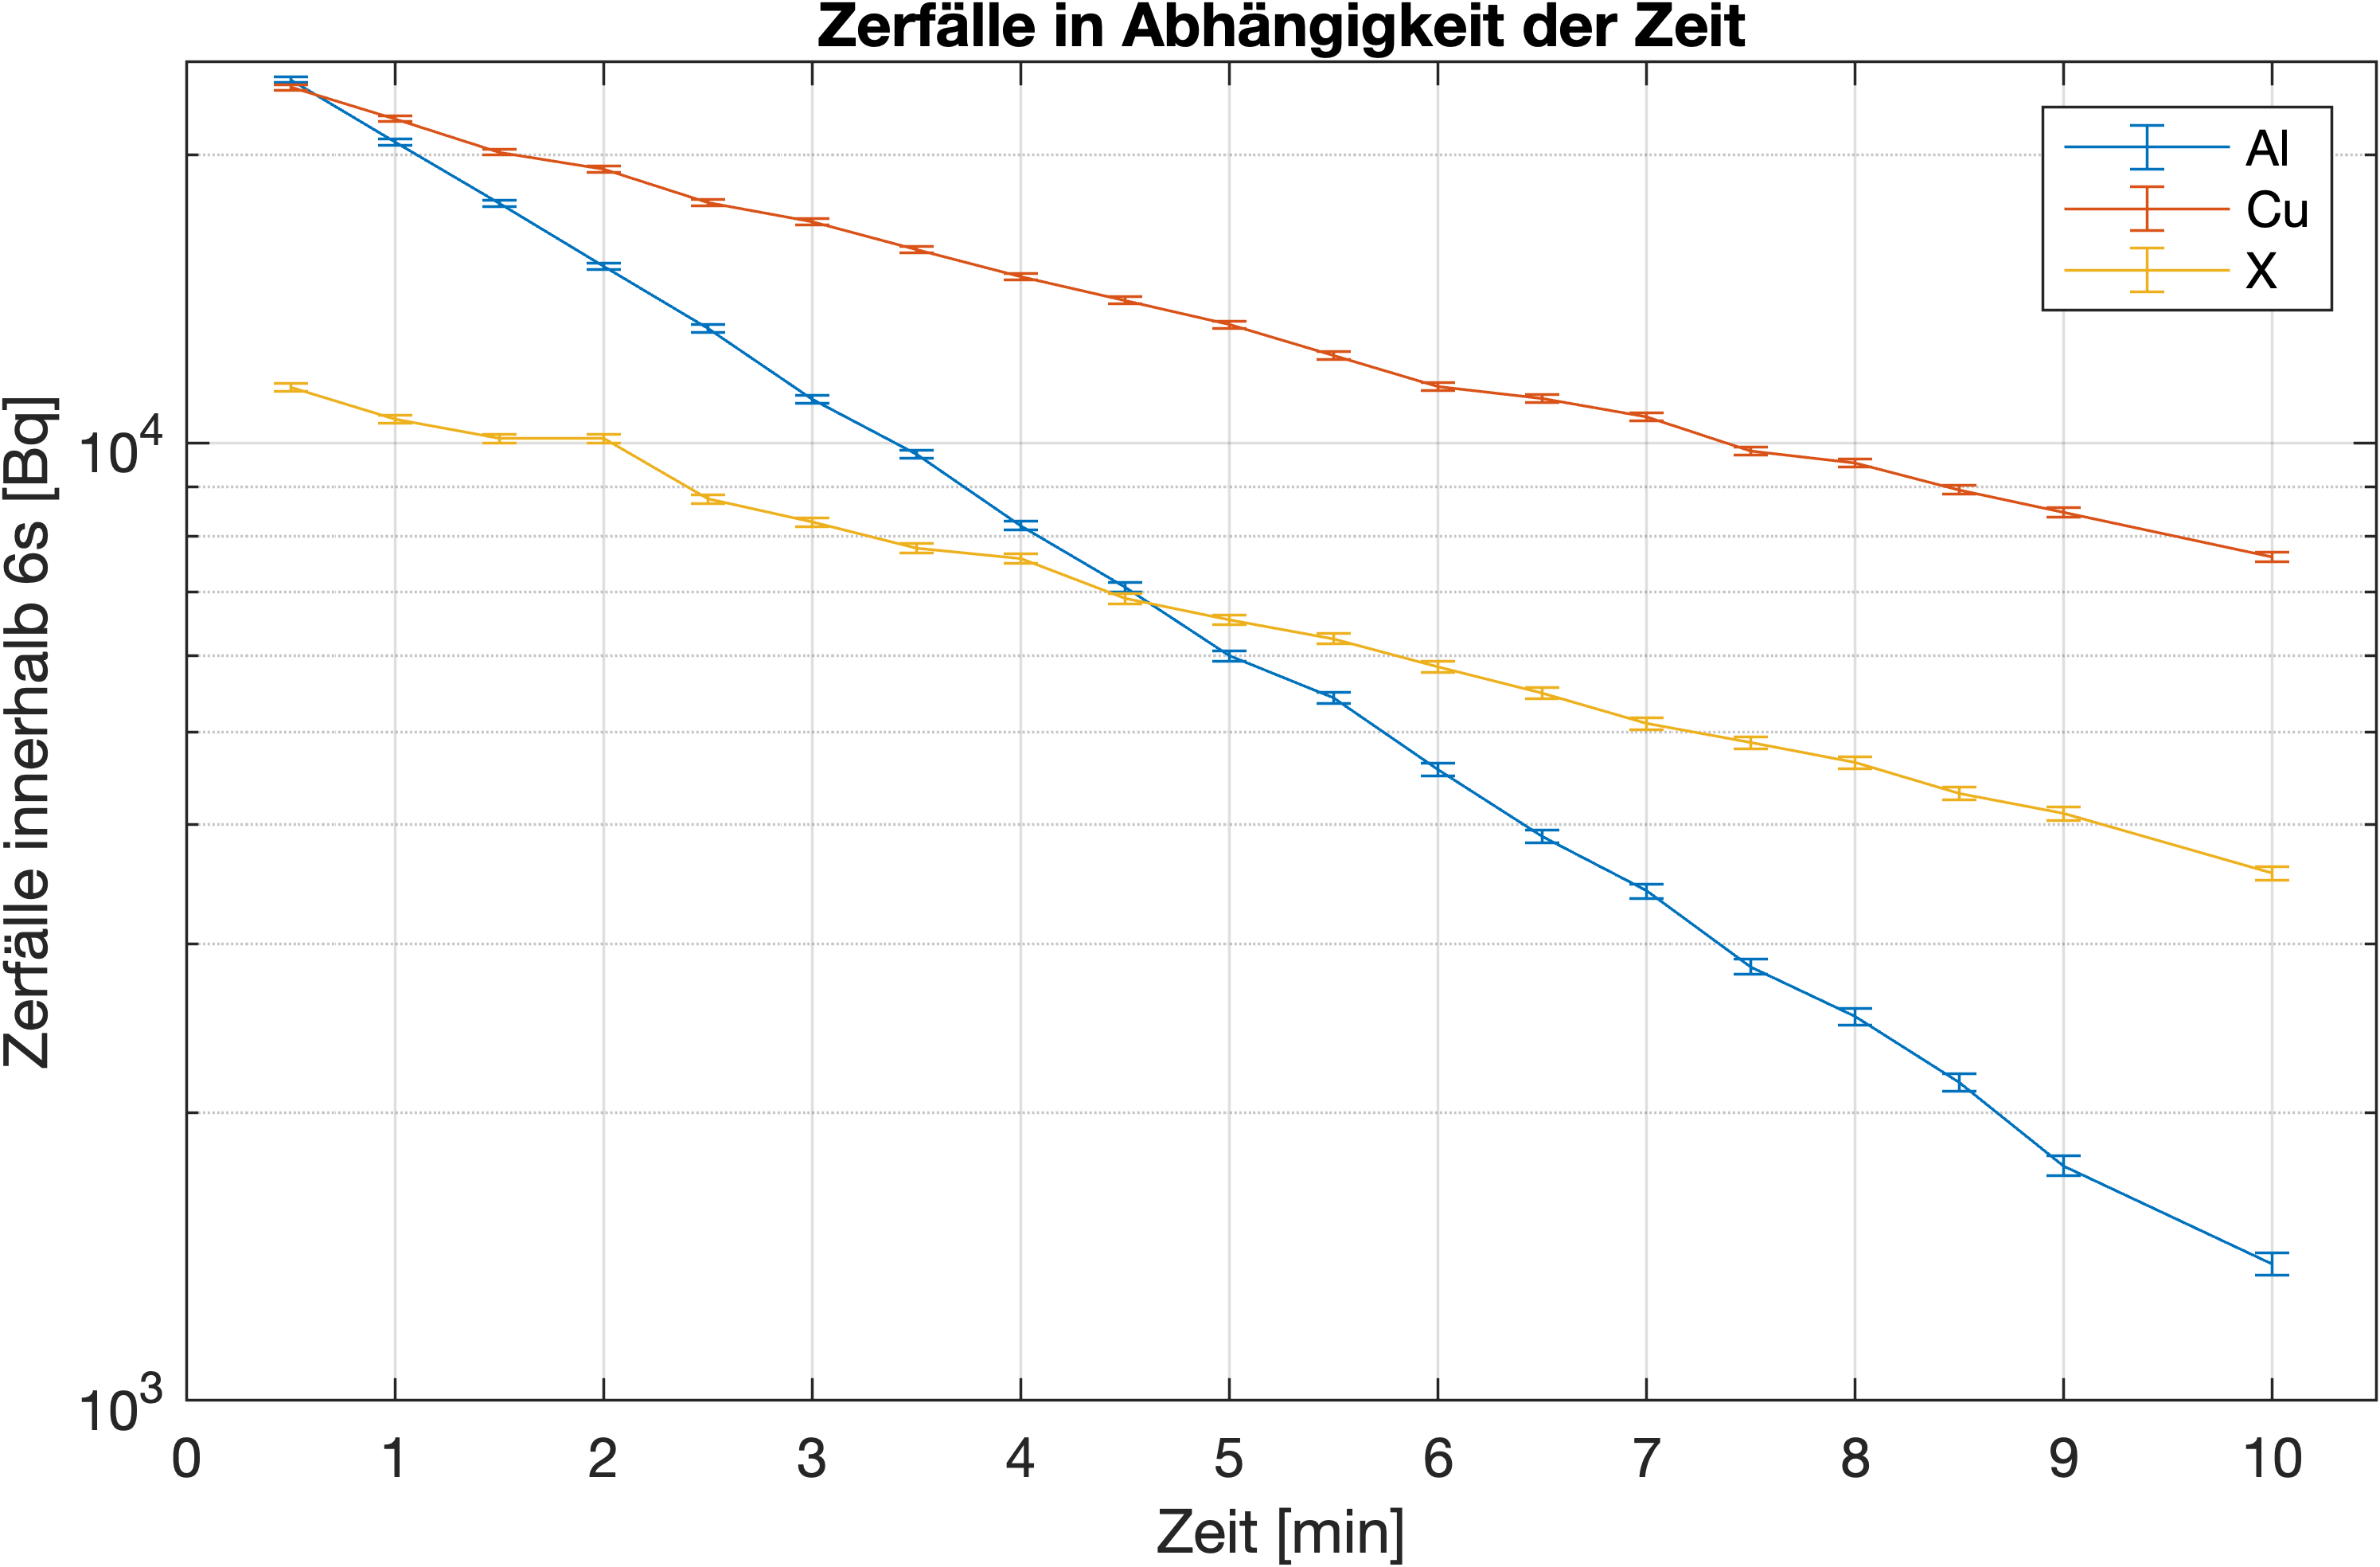
\includegraphics[width=\textwidth]{logarithmic.png}
        \caption{Messwerte mit logarithmischer Achse}
    \end{figure}

    \section{Bestimmung der Halbwertszeiten}
    \noindent
    Anhand der Abklingkurven kann man nun die Halbwertszeiten ablesen. \\
    Da der Verlauf der Aktivitätswerte durch den radioaktiven Zerfall einer Exponentialfunktion folgt, kann diese mittels exponentieller Regression näherungsweise bestimmt und anschließend die Halbwertszeit errechnet werden.
    Die aus den gemessenen Aktivitätswerten resultierenden Exponentialfunktionen sind folgende:
    \begin{align*}
        y_\text{Al} &= e^{10.2344\, -\, 0.3021 \cdot x} \\
        y_\text{Cu} &= e^{10.0940\, - \, 0.1182 \cdot x} \\
        y_\text{X} &= e^{9.3969\, -\, 0.1210 \cdot x}
    \end{align*}
    Nach der Bestimmung der Umkehrfunktionen lassen sich die Halbwertszeiten wie folgt berechnen:
    \begin{equation*}
        T_{1/2} = y^{-1}\left(\frac{y(100)}{2}\right) - 100
    \end{equation*}
    Die damit berechneten Halbwertszeiten lauten:
    \begin{align*}
        T_{1/2;\, \text{Al}}&: 2.29\, \text{min} \\
        T_{1/2;\, \text{Cu}}&: 5.86\, \text{min} \\
        T_{1/2;\, \text{X}}&: 5.72\, \text{min}
    \end{align*}
    Die Linie der Zerfallskurve der unbekannten Probe in der logarithmischen Darstellung verläuft nahezu parallel zur Zerfallskurve der Kupferprobe.
    Damit lässt sich vermuten, dass es sich bei der unbekannten Probe ebenfalls um ein Kupfergemisch handelt, in welchem das Isotop \(^{66}\)Cu wiederum die niedrigste Halbwertszeit, und damit, für die gemessene Zeitspanne, den größten Einfluss besitzt. \\
    Das durchschnittliche Verhältnis der Impulsrate der unbekannten Probe zur Impulsrate der Kupferprobe beträgt ca. \(0.49\). Daraus lässt sich schließen, dass der Kupferanteil im unbekannten Gemische ungefähr bei der Häflte liegt. \\
    Zur weiteren Bestimmung der unbekannten Probe wäre eine Impulsmessung über einen längeren Zeitraum hinweg notwendig, um Halbwertszeiten anderer Gemischbestandteile auswerten zu können. \\
    Auf Grundlage einer visuellen Beurteilung sowie eines Hinweises seitens des Versuchsleiters, wird hinter der unbekannten Probe die Kupfer-Zink-Legierung Messing vermutet, welches wie gefordert zu ca. 50\% aus Kupfer besteht, sowie mit Zink einen zweiten Gemischbestandteil hoher Halbewertszeit besitzt.
    \section{Berechnen der Neutronenflussdichte am Bestrahlungsort}
    Nach Versuchsanleitung ergibt sich zur Berechnung der Neutronenflussdichte am Bestrahlungsort folgende Gleichung:
    \begin{equation*}
        \Phi = \frac{\left(\text{Z}(t_b)\, -\, n_0\right) \cdot \text{AG}}{C \cdot V \cdot \rho \cdot P \cdot N_L \cdot \sigma \cdot \left[1 - \exp(-\ln(2)/T_{1/2} \cdot t_b)\right]}
    \end{equation*}
    \begin{align*}
        Z(t_b) &: \text{(extrapolierte Zählrate für $t = 0$ = $t_b$)} \\
        n_0 &: \text{Nulleffekt} \\
        AG &: \text{Atomgewicht des Probenmaterials} \\
        C &: \text{Proportionalitätsfaktor für Fehlerquellen (für Kupfer bestimmt: 0,01)} \\
        V &: \text{Volumen der bestrahlten Materialprobe} \\
        \rho &: \text{Dichte des bestrahlten Materials} \\
        P &: \text{Anteil des betrachteten Isotops am Gemisch (für Kupfer: 0.309)} \\
        N_L &: \text{Loschmidtsche Zahl} \\
        \sigma &: \text{mikroskopischer Wirkungsquerschnitt} \\
        T_{1/2} &: \text{expermientell ermittelte Halbertszeit} \\
        t_b &: \text{Dauer der Aktivierung im Reaktor} \\
    \end{align*}
    Damit lässt sich für Aluminium eine Neutronenflussdichte berechnen mit:
    \begin{align*}
        \Phi_{\text{Al-28}} &= \frac{\left(4640.79\, \frac{1}{\text{s}} - 89.66\, \frac{1}{\text{s}}\right) \cdot 27\, \frac{\text{g}}{\text{mol}}}{0.01 \cdot 0.71\, \text{cm}^3 \cdot 2.2\, \frac{\text{g}}{\text{cm}^3} \cdot 6.025 * 10^{23}\, \frac{1}{\text{mol}} \cdot 0.215 * 10^{-24}\, \text{cm}^2 \cdot \left[1 - \exp\left(- \frac{\ln(2)}{2.29\, \text{min}} \cdot 10\, \text{min}\right)\right]} \\
            &= 6.412 \cdot 10^7\, \frac{\text{n}}{\text{cm}^2 \cdot \text{s}}
    \end{align*}
    sowie für Kupfer mit:
    \begin{align*}
        \Phi_{\text{Cu-66}} &= \frac{\left(4032.9\, \frac{1}{\text{s}} - 89.66\, \frac{1}{\text{s}}\right) \cdot 65\, \frac{\text{g}}{\text{mol}}}{0.01 \cdot 0.71\, \text{cm}^3 \cdot 8.92\, \frac{\text{g}}{\text{cm}^3} \cdot 0.309 \cdot 6.025 * 10^{23}\, \frac{1}{\text{mol}} \cdot 2.1 * 10^{-24}\, \text{cm}^2 \cdot \left[1 - \exp\left(- \frac{\ln(2)}{5.86\, \text{min}} \cdot 10\, \text{min}\right)\right]} \\
            &= 1.499 \cdot 10^7\, \frac{\text{n}}{\text{cm}^2 \cdot \text{s}}
    \end{align*}
    Die berechneten Werte liegen damit wie erwartet in der für Nullleistungsreaktoren gegebenen Größenordnung von \(10^7 \frac{\text{n}}{\text{cm}^2 \cdot \text{s}}\).

\end{document}